\documentclass[border=2pt]{standalone}
\usepackage{times}
\usepackage{amsmath,amssymb}
\usepackage{tikz}
\usetikzlibrary{arrows.meta,calc,positioning}
\begin{document}
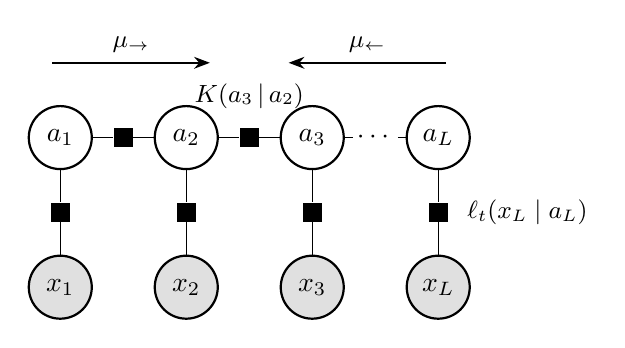
\begin{tikzpicture}[
    var/.style={circle,draw,thick,minimum size=8mm,inner sep=0pt},
    obs/.style={circle,draw,thick,fill=black!12,minimum size=8mm,inner sep=0pt},
    fac/.style={rectangle,fill=black,minimum size=2.4mm,inner sep=0pt},
    lab/.style={font=\small}]
  \foreach \i/\n in {0/1,1/2,2/3,3/L} {
    \node[var] (a\i) at (1.6*\i,0) {$a_{\n}$};
    \node[fac] (o\i) at (1.6*\i,-0.95) {};
    \node[obs] (x\i) at (1.6*\i,-1.9) {$x_{\n}$};
    \draw (a\i) -- (o\i) -- (x\i);
  }
  \foreach \i/\j in {0/1,1/2} {
    \node[fac] (k\i) at ($(a\i)!0.5!(a\j)$) {};
    \draw (a\i) -- (k\i) -- (a\j);
  }
  \draw (a2) -- ($(a2)!0.32!(a3)$);
  \node at ($(a2)!0.5!(a3)$) {$\cdots$};
  \draw ($(a2)!0.68!(a3)$) -- (a3);
  \node[lab,above=1.2mm of k1] {$K(a_3\,|\,a_2)$};
  \node[lab,right=1.2mm of o3] {$\ell_t(x_L\mid a_L)$};
  \draw[-{Stealth[length=2mm]},thick] ($(a0)+(-0.1,0.95)$) -- node[above,lab]{$\mu_{\to}$} ($(a1)+(0.3,0.95)$);
  \draw[-{Stealth[length=2mm]},thick] ($(a3)+(0.1,0.95)$) -- node[above,lab]{$\mu_{\leftarrow}$} ($(a2)+(-0.3,0.95)$);
\end{tikzpicture}
\end{document}
